\documentclass[runningheads]{llncs}

\usepackage{tikz}
\usepackage{tikz-qtree}
\usepackage{graphicx}
\usepackage{amsmath}
\usepackage{mathtools}
\usepackage{array}
\usepackage{algorithm}
\usepackage[noend]{algpseudocode}
\usepackage{graphicx}
\graphicspath{{./}}

\begin{document}

% \thanks{Supported by organization x.}
\title{Semantic Genetic Programming on the GPU}
\author{João David\inst{1} \and
Ye Yang\inst{1}
}
%\authorrunning{F. Author et al.}

\institute{Departamento de Informática da Faculdade de Ciências da Universidade de Lisboa
\email{\{fc49448,fc49521\}@alunos.fc.ul.pt}}

\maketitle

\begin{abstract}
Semantic Genetic Programming, also known as Semantic GP, is a type of Evolutionary Algorithm (EA), a subset of machine learning. 
Aiming to not only syntactically manipulate the data to promote a better fitness evaluation, but also ensuring that the resulting function is semantically correct. Traditional implementations of genetic programs have always been done on CPU, taking advantage of its multiple cores to do parallel work. We aim to improve on the parallelization of the genetic algorithm by implementing it on the Graphics Processing Unit (GPU), taking advantage of its vast amount of processing cores, which are multiple times that of the CPU. The implementation will be done on an NVidia GPU allowing the use of the Compute Unified Device Architecture (CUDA) API, which grants us access to directly manipulate the GPU memory and threads necessary to perform fitness evaluation and crossover.


\keywords{Genetic Programming  \and GPU \and CUDA \and Machine Learning.}
\end{abstract}
%
%
%
\section{Introduction}

Traditional implementations of Semantic GP are  on CPU, usually with syntax trees that contain elements of the domain in study, whether it be logical operations, mathematical operations, among others.

These trees are then processed given some input, and the output is compared to some target value to calculate its fitness. Fitness calculation algorithms are generally implemented on CPU, in this paper we aim to vastly improve the time required computing and evaluating fitness values by implementing an algorithm on GPU, taking advantage of its many cores and threads which allows for a vast amount of parallel computation to be done, when compared to a CPU.

In section 2 we explain some of the main concepts needed to understand the parallel implementation of fitness testing, in section 3 we discuss the general approach taken to parallelize fitness evaluation, which can be applied to any programming. In section 4 we explain in more detail our implementation which is written in C with a CUDA extension, allowing us to fully utilize all the functionality provided by the API. In section 5 we compare test results from both a parallel and sequential implementations of the algorithm. In section 6 we discuss previous work done on the subject matter and compare it with our own implementation and finally we summarize all the findings in the paper and future work to be done in section 7.

With this paper we aim to:
\begin{itemize}
	\item To propose a parallel algorithm implemented on the GPU using the CUDA API for Semantic Genetic Programming
	\item compare execution times of the implemented algorithm with a sequential CPU version
\end{itemize}


\section{Background}

Genetic Algorithms are inspired by Nature and its biological mechanisms, take the following analogy as an example. Imagine that you are in the horse racing business, and you own a set of horses (population), some horses are better at different skills (speed, resistance, strength, etc.). When selecting horses to produce offspring (crossover and mutation), you must select them based on their fitness, which is calculated using a fitness function. In this case, it could be the average lap time from a set of tracks, better fitness values would mean lower average lap times.

The semantic syntax our work will be based on will be presented as a tree structure, each node containing either a mathematical operator, a literal or a variable which can be swapped by a value from a given data set.
When processing a tree through a data set row, each variable will be swapped by the corresponding value in the data set according to the variable column index. In Figure \ref{syntree} we can see the tree representation of the mathematical formula $x0 * (x1+4)$ which is then processed according to a data set row containing the values $(0.5\quad 25.3\quad 6.2\quad 12)$. The values within the data set that are not referenced by any variable in the tree are ignored.
\begin{figure}

\hfil
\begin{tikzpicture}
  \Tree [.* [.x0 ] 
             [.+ [.x1 ] [.4 ]]]
  %
  \begin{scope}[shift = {(5cm, 0cm)}]
  \Tree [.* [.$0.5$ ]  
            [.+ [.$25.3$ ] [.4 ]]]
  \end{scope}
  %
  \draw[->, yshift = -1.5cm] (2, 0) -- (3, 0);
\end{tikzpicture}
\hfil
\caption{Syntax tree value swap example}
\label{syntree}
\end{figure}


An NVIDIA GPU is composed of several SM (Stream Multiprocessor), each SM having a certain amount of cores, every core contains a number of warps (groups of 32 threads).
The processing in an NVIDIA GPU is done through the use of blocks, which are composed of a set amount of threads. Each block will be scheduled to a single SM, and every SM can schedule different blocks at a given time if it has enough resources. When choosing the number of threads within a block, it is important that the number is a multiple of 32. Because if it isn't, there will be threads of a warp doing nothing.

Neither GPUs nor CPUs can directly access each others memory space. In order to cooperate, it is required to have copied memory from RAM to GPU memory (GDRR5 for instance) in order for GPUs to process data. Then the processed data must be copied back to RAM, so that the CPU may access it.

To execute a method on the GPU, we have to execute a kernel call. The kernel call can receive up to 3 parameters between the \texttt{<<< >>>} brackets. The first two parameters determine the number of blocks and threads per block respectively and the last one determines the amount of shared memory between threads available (threads can only access shared memory content within the same block) in bytes, when omitted it defaults to 0.

\section{Approach}
The algorithm starts by generating N trees, and then processing them based on the data set values. For each tree and for each row, there is an output value $V_{i,j}$, where \textit{i} is the tree index, and \textit{j} the row index (row number - 1) in the data set file.
The Fitness ($F_i$) for each tree is then calculated using the Mean Squared Error (MSE) and stored in an array of size N indexed by the tree index. $Y_j$ is the target value of row's number \textit{j}. $$F_i = \frac{1}{N}\sum_{i=1}^{N} (V_{i,j} - Y_j)^{2}$$

After that, a matrix $A$[G$\times$N] is created, where G is the number of generations, $a_{i,j}$ is the tree index with which the tree \textit{j} crossed over with at generation \textit{i}.
\begin{equation*}
A_{G,N} = 
\begin{bmatrix}
0 & 1 & \cdots & N-1 \\
a_{2,1} & a_{2,2} & \cdots & a_{2,N} \\
\vdots  & \vdots  & \ddots & \vdots  \\
a_{G,1} & a_{G,2} & \cdots & a_{G,N} 
\end{bmatrix}
\end{equation*}

For every odd generation cycle, trees will be divided in two groups, one group with odd index and the other with even index, trees only crossover trees within the same group.

For every even generation cycle, trees will be divided in two groups, one group with index $<$ N/2 and the other with index $\geq$ N/2, trees only crossover trees within the same group.

The fitness array obtained from the previous iteration will be split in two groups, (based on the current generation cycle) in the same way mentioned above, the index of the best fitness from each group will be the tree index that all the trees from the same group will crossover with.

When a tree \textit{a} is crossing over with a tree \textit{b}, the result of said crossover will be stored in a new fitness array at \textit{a}'s index. The result would be:$$newFitness[a_{index}] = oldFitness[a_{index}] + sigmoid(oldFitness[b_{index}])$$

Given this alternating crossover algorithm, we can achieve a less linear evolution from generation to generation. Algorithm~\ref{crossover_alg} is a pseudo code representation of the algorithm.

\begin{algorithm}
\caption{Tree crossover}
\begin{algorithmic}[1]
\Procedure{TreeCrossover}{}
\State \textbf{int[G][N]} \textit{A}
\State \textbf{float[N]} \textit{oldFitness}
\State \textbf{float[N]} \textit{newFitness}
\For{$i = 0;\ i < N;\ i++$}
	\State {A[0][i] = i}
\EndFor
\For{$gen = 1;\ gen < G;\ gen++$}
\If {$\textit{gen} \ \%\ 2 	\neq 0$}
	\State \textbf{int} \textit{bestFitOdd}
	\State \textbf{int} \textit{bestFitEven} 
	\For{$i = 0 ;\ i < N;\ i++$}
		\State {find best fitness with odd index and store it in \textit{bestFitOdd}}
		\State {find best fitness with even index and store it in \textit{bestFitEven}}		
	\EndFor
	\State A[gen][odd indexes] = bestFitOdd
	\State A[gen][even indexes] = bestFitEven
\Else
	\State \textbf{int} \textit{bestFitFirstHalf}
	\State \textbf{int} \textit{bestFitSecondHalf}
	\For{$i = 0 ;\ i < N;\ i++$}
		\State {find best fitness with index $<$ N/2 and store it in \textit{bestFitFirstHalf}}
		\State {find best fitness with index $\geq$ N/2 and store it in \textit{bestFitSecondHalf}}		
	\EndFor
	\State A[gen][index $<$ N/2] = bestFitFirstHalf
	\State A[gen][index $\geq$ N/2] = bestFitSecondHalf
\EndIf
\For{$i = 0 ;\ i < N;\ i++$}
	\State newFitness[i] = oldFitness[i] + sigmoid(oldFitness[A[gen][i])
\EndFor
\EndFor
\EndProcedure
\end{algorithmic}
\label{crossover_alg}
\end{algorithm}


\section{Implementation Details}
Before any values could be first calculated, we needed some form of input to compare values with. This lead to the implementation of a data set parser. The data set is a text file in which all the variables and target values are defined. Each line has an equal amount of values \textit{Y} written, the last of which corresponds to the target value. Both variable values and target values are then extracted and stored in separate arrays which will be used to calculate the fitness for the first generation of trees.

To store and calculate the values, a set number of random syntax trees have to be initially generated. Each node of the tree as previously mentioned can be a literal value, a variable or a mathematical operator. After generating the trees, each one of them must be run through the data set to evaluate its fitness by calculating the mathematical operations defined and comparing it with the target values. The computation is handled as a Reverse Polish Notation calculator (RPN) according to the following procedures:
\begin{itemize}
	\item A separate LIFO stack to store literal values and variables is created
	\item The tree is traversed in postorder so that the root operation or value is read last
	\item If either a literal or a variable are present, they are pushed into the stack
	\item If a mathematical operation is read, 2 values are popped out of the stack for computing, and the resulting value is pushed back into the stack
	\item At the end of the processing, the final value is popped from the stack and stored in a result matrix of size $N_{trees}*dataset_{rows}$ with each row representing the calculated values for a given data set row by a syntax tree and each column the resulting values to compare with the target values.
\end{itemize}

\subsection{GPU Parallelization}
Just like mentioned in the Approach section, after processing the trees based on the data set values, we are left with a set of $V_{i,j}$ values. We will use the GPU to perform a reduction (Figure~\ref{fitness_calc}), obtaining the Mean Squared Error, which will be the initial fitness value.

In Figure~\ref{fitness_calc} we present an example of initial fitness calculation with a data set of 4 lines, meaning that each tree computes 4 different $V_{i,j}$ values which are compared to the 4 target values $Y_j$ to determine the MSE and consequently the fitness of the tree. Each tree is processed by a block with the number of threads being the same as the number of lines (4 in this case) which will have its own ID that can be extracted with the built in keyword \textit{blockIdx.x}. The \textit{.x} termination means we are extracting the ID along the \textit{x} axis, since the kernel is launched in 1 dimension, both the \textit{y} and \textit{z} values are 0.

$V_{i,j}$ is the value calculated by a tree of index \textit{i} on row index \textit{j} of the data set and $Y_{j}$ the respective target value. Each $(V_{i,j} - Y_{j})^{2}$ value is calculated by a single thread.

After all values are calculated we then proceed to a reduction phase, in this phase the amount of threads working on adding up all the values is reduced by half with each step until it reaches 1 (\textit{threadId.x} $<$ 1), which will be the final value to be divided by \texttt{num\_rows} resulting in the MSE, which will be the fitness value for the tree with index equal to \textit{blockId.x}. Since all blocks work in parallel, the complexity of the reduction algorithm is $O(log(n))$.

After calculating the initial fitness for all trees, we can then proceed apply the GPU version of the algorithm described in Algorithm 1. Due to the way the algorithm is implemented, the correct partitioning of the array in blocks can be achieved only if the number of trees is a power of 2.

The default value for the number of threads per block is 512 (multiple of 32), the number of blocks to be launched is then calculated by dividing the number of trees by 512 (threads per block).

We then perform a reduction using the kernel call of the method \texttt{gpu\_phase\_one}, each block will find the best fitness and its corresponding index in the fitness array previously calculated within the following indexes of said array: $$[\textit{blockDim.x} * \textit{blockIdx.x} + 0; \textit{blockDim.x} * \textit{blockIdx.x} + 512[$$
After this, we need to synchronize all blocks in order to find the best fitness and its index in the fitness array by comparing the results from each block. We do this by using another kernel call \texttt{gpu\_phase\_two} with the same blocks/threads per block as the previous one. This kernel call will look up the values written to the auxiliary arrays \texttt{dev\_fitness\_aux} and \texttt{dev\_fitness\_index\_aux} by the \texttt{gpu\_phase\_one} kernel call. The values are written and read from said arrays based on whether the current generation is odd or even.

For odd generation cycles, every odd threadIdx.x from all blocks will find the best fitness value by only looking up odd indexes of the auxiliary arrays, while even threadIdx.x will do the same but for even indexes of said auxiliary arrays.

For even generation cycles, blocks with blockIdx.x $<$ gridDim.x/2 will find the best fitness value by only looking up indexes $<$ gridDim.x/2 on the auxiliary arrays, while blocks with blockIdx.x $\geq$ gridDim.x/2 will do the same but for indexes $\geq$ gridDim.x/2.

After finding the best fitness \textit{x} and the corresponding index \textit{i}, every thread of every block will write to the $A_{G,N}$ matrix the index of the tree with the best fitness, and then will write to the \texttt{new\_fitness} array the fitness of crossing over the tree at indexes threadIdx.x and \textit{i}, using the fitness value of the tree threadIdx.x from the previous fitness array plus the sigmoid of the best fitness value just discovered, \textit{x}.

Then a new generation will start, where the \texttt{new\_fitness} will now be the previous fitness array. Once all the generations have passed, the values in the matrix $A_{G,N}$ and \texttt{new\_fitness} will be copied to RAM.

\begin{figure}[!htb]
\begin{center}
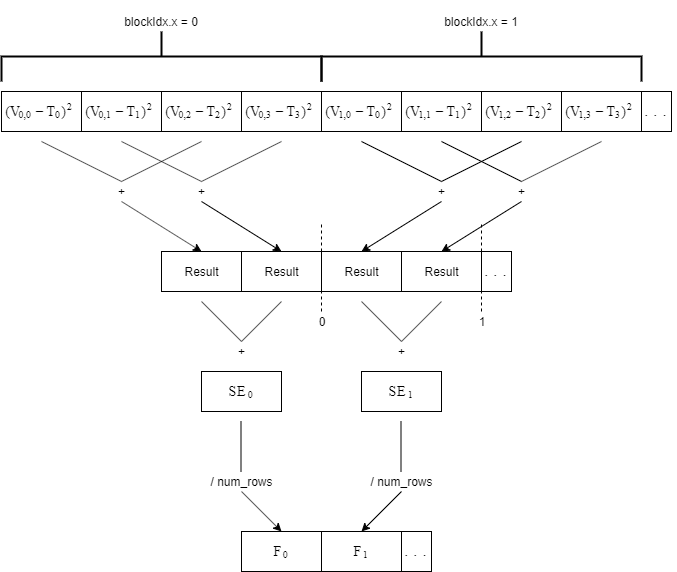
\includegraphics[scale=0.35]{Fitness_Calculation1}
\end{center}
\caption{Fitness computation for a data set of 4 lines}
\label{fitness_calc}
\end{figure}

\section{Evaluation}

\subsection{Experimental Setup}

\begin{center}
 \begin{tabular}{|>{\centering\arraybackslash}p{4cm}|>{\centering\arraybackslash}p{2cm}|>{\centering\arraybackslash}p{2cm}|>{\centering\arraybackslash}p{2cm}|} 
 \hline
 Processor & CPU Cores & Threads & RAM \\ [0.5ex] 
 \hline\hline
 Intel Xeon X5670 & 12 & 24 & 24GB \\
 \hline
\end{tabular}
\end{center}

\begin{center}
\begin{tabular}{|>{\centering\arraybackslash}p{4cm}|>{\centering\arraybackslash}p{2cm}|>{\centering\arraybackslash}p{2cm}|>{\centering\arraybackslash}p{2cm}|}
 \hline
 Graphics Card & GPU Cores & CUDA Capability & GDDR5 Memory \\ [0.5ex] 
 \hline\hline
 NVidia GTX 960 & 1024 & 5.2 & 4GB\\  
 \hline
\end{tabular}
\end{center}

In this section you should describe the machine(s) in which you are going to evaluate your system. Select the information that is relevant.


\subsection{Results}

In this section you should present the results. Do not forget to explain where the data came from. 

You should include (ideally vectorial) plots, with a descriptive caption. Make sure all the plots (Like Figure~\ref{fig1} are well identified and axis and metrics are defined.

\subsection{Discussion}

Here you should discuss the results on a high level. For instance, based on our results, the parallelization of the merge-sort is relevant as no other parallel work occurs at the same time, and the complexity $O(Nlog(N))$ can have a large impact when the number of individuals is high.

\section{Related Work}

Alberto Moraglio, Krzysztof Krawiec, and Colin G. Johnson introduced a new way of genetic programming, Geometric Semantic Genetic Programming (GSGP) which consists in changing the semantics of the functions directly. Their work in regards to fitness evaluation, tree mutation and crossover is far more complex than ours given that we only accounted for mutation by concatenation with sums of trees. However the implementation of the genetic algorithm was done on CPU which makes performance considerably slower if it were implemented on GPU.


\section{Conclusions}

In this paper, we proposed a parallel GPU algorithm to both calculate and evaluate fitness on a genetic program, by applying 2 different crossover techniques. We concluded that GPU parallelization significantly benefits the execution time when passing from one generation to the next, by dynamically distributing work across the many GPU threads available. However, the size of the initial data set must be taken into account, as smaller data sets may be quicker to compute on the CPU due to the significant overhead when transitioning from CPU memory to GPU memory. Thus we must define a cutoff mechanism between CPU and GPU execution which can be determined in future tests.

We presented a simple crossover algorithm when passing from one generation to the next, in future work we would like to implement tree mutations and crossover between trees rather than the fitness calculated with each passing generation. The implementation of a CPU parallel version of the algorithm would also compliment the results obtained in this paper, so a comparison between the two parallel frameworks can be made.

\section*{Acknowledgements}

João David wrote the sequential version of the algorithm and two GPU methods, while Ye Yang wrote the other GPU method, the data set parser and the tree processing.

Both authors wrote this paper, with João David focusing on the approach and introduction while Ye Yang focused on implementation details, related work and conclusion.

Each author spent around 40 hours on this project.

\bibliographystyle{splncs04}
\bibliography{bibliography}

\end{document}
